\documentclass{aip-cp}
\usepackage{listings}
\usepackage[numbers]{natbib}
\usepackage[only,llbracket,rrbracket,llparenthesis,rrparenthesis]{stmaryrd}
\usepackage{graphicx}
\usepackage{amsmath}
\usepackage{amssymb}
\usepackage{txfonts}
\usepackage[utf8]{inputenc}

\begin{document}
\title{The Systems Engineering of Consistent Pure Language \\
       with Effect Type System \\
       for Certified Applications and Higher Languages}

\author[aff1]{Maksym Sokhatskyi\corref{cor1}}
\eaddress[url]{https://groupoid.space}
\author[aff1]{Pavlo Maslianko\corref{cor3}}

\affil[aff1]{National Technical University of Ukraine ``Igor Sikorsky Kyiv Polytechnical Institute''}
\corresp[cor1]{maxim@synrc.com}
\corresp[cor3]{mppdom@i.ua}

\maketitle
\vspace{1cm}
\begin{abstract}
This paper presents the design of the {\bf Om} language and an implementation of its type checker and bytecode extractor to Erlang.
Om is an intermediate language based on a pure type system with the infinite number of universes, so it is known to be consistent in dependent type theory.
The type checker can be switched between predicative and impredicative hierarchies of universes.
The need to natively support Erlang platform dictated the look and feel of this work.
This system is expected to be usable as trusted core for certified applications which could be run inside Erlang virtual machines LING and BEAM.
The syntax is compatible with Morte language and supports its base library, however, it extends the indexed universes.
We show how to program in this environment and link with Erlang inductive and coinductive free structures.
A very basic prelude library is shipped as a part of the work.
We briefly describe the top-level language which compiles to pure type system core.
As the results, we will show lambda evaluation performance on BEAM virtual machine.
\end{abstract}

\section{Introduction}
IEEE\footnote{IEEE Std 1012-2016  --- V\&V Software verification and validation} standard
and ESA\footnote{ESA PSS-05-10 1-1 1995 -- Guide to software verification and validation} regulatory documents define a number of tools and approaches for verification and validation processes. 
The most advanced techniques involve mathematical languages and notations. 
The age of verified math was started by de Bruin's AUTOMATH prover and Martin-Löf\cite{Lof84}'s type theory. 
Today we have Coq, Agda, Lean, Idris, F* languages which are based on Calculus of Inductive Constructions or CiC\cite{Mohring15}.
The core of CiC is Calculus of Constructions or CoC\cite{Coq88}.
Further development has lead to Lambda Cube\cite{Henk93} and Pure Type Systems by Henk\cite{Erik97} and Morte\footnote{Gabriel Gonzalez. Haskell Morte Library}.
Pure Type Systems are custom languages based on CoC with single Pi-type and possibly other extensions.
Notable extensions are ECC, ECC with Inductive Types\cite{Ore92}, K-rules\cite{Barthe95}.
The main motivation of Pure Type Systems is an easy reasoning about core, strong normalization and trusted external verification due to compact type checkers.
A custom type checker can be implemented to run certified programs retrieved over untrusted channels.
The applications of such minimal cores are 1) Blockchain smart-contract languages, 2) certified applications kernels, 3) payment processing, etc.

\subsection{Generating Trusted Programs}
According to Curry-Howard, a correspondence inside Martin-Löf Type Theory\cite{Lof84} proofs or certificates are lambda terms of particular types or specifications.
As both specifications and implementations are done in a typed language with dependent types we can extract target implementation of a certified program just in any programming language.
These languages could be so primitive as untyped lambda calculus and are usually implemented as untyped interpreters (JavaScript, Erlang, PyPy, LuaJIT, K).
The most advanced approach is code generation to higher-level languages such as C++ and Rust (which is already language with trusted features on memory, variable accessing, linear types, etc.).
In this work, we present a simple code extraction to Erlang programming language as a target interpreter.
However, we have also worked on C++ and Rust targets as well.

\subsection{System Architecture}
{\bf Om} as a programming language has a core type system, the {\bf PTS$^{\infty}$} --- the pure type system with the infinite number of universes.
This type system represents the core of the language.
Higher languages form a set of front-ends to this core.
 Here is example of possible languages:
1) Language for inductive reasoning, based on CiC with extensions;
2) Homotopy Core with interval [0,1] for proving J and funExt;
3) Stream Calculus for deep stream fusion (Futhark);
3) Pi-calculus for linear types, coinductive reasoning and runtime modeling (Erlang, Ling, Rust).
These languages desugar to {\bf PTS$^{\infty}$} as an intermediate language before extracting to target language\footnote{Note that extracting from [0,1] Homotopy Core is an open problem}.

Not all terms from higher languages could be desugared to PTS.
As was shown by Geuvers\cite{Geuvers01} we cannot build induction principle inside PTS, we need a fixpoint extension to PTS.
And also we cannot build the J and funExt terms.
But still PTS is very powerful, it's compatible with System F libraries.
The properties of that libraries could be proven in higher languages with Induction and/or [0,1] Homotopy Core.
Then runtime part could be refined to PTS, extracted to target and run in an environment.

We see two levels of extensions to PTS core: 1) Inductive Types support; 2) Homotopy Core with [0,1] and its eliminators.
We will touch a bit this topic in the last section of this document.

\begin{figure}[h]
  \centerline{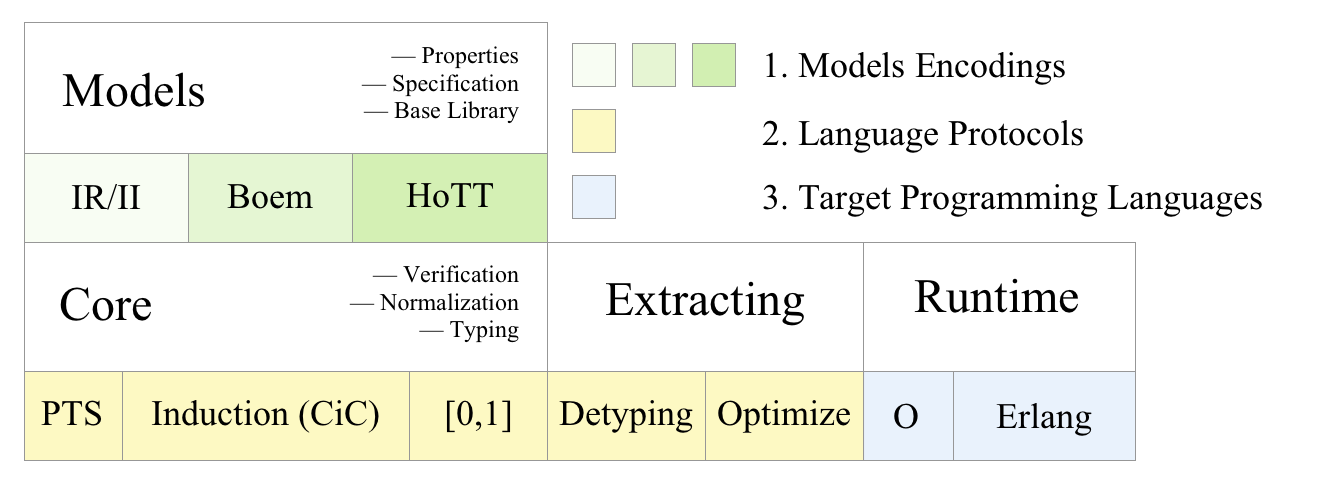
\includegraphics[scale=0.28]{static}}
  \caption{The Systems Engineering of Model Verifications}
\end{figure}

\subsection{Place among other languages}
The product is a regular Erlang/OTP application, that provides dependent language services to the Erlang environment: 1) type checking; 2) normalization; 3) extraction.
All parts of {\bf Om} compiler is written in Erlang language and target/runtime language is Erlang.

\begin{itemize}
\item Level 0 --- certified vectorized interpreter
\item {\bf Level 1 --- consistent pure type system for type checking and normalization}
\item Level 2 --- higher language for theorem proving and models property checking
\end{itemize}

\begin{table}[h]
\caption{List of languages, tried as verification targets}
\label{tab:a}
\tabcolsep7pt\begin{tabular}{lcccc}
\hline
\tch{1}{c}{b}{Target Language} & \tch{1}{c}{b}{Class} & \tch{1}{c}{b}{Higher\\ Language} & \tch{1}{c}{b}{Type\\ Theory}\\
\hline
C++        & compiler/native      & HNC & System F\\
Rust       & compiler/native      & HNC & System F\\
JVM        & interpreter/native   & Java    & F-sub\footnote{System F wit bounded quantification}\\
JVM        & interpreter/native   & Scala   & System F-omega\\
GHC Core   & compiler/native      & Haskell & System D\\
GHC Core   & compiler/native      & Morte   & CoC\\
Haskell    & compiler/native      & Coq     & CiC\\
OCaml      & compiler/native      & Coq     & CiC\\
{\bf BEAM} & {\bf interpreter} & {\bf Om}   & {\bf PTS$^\infty$} \\
O          & interpreter          & Om  & PTS$^\infty$ \\
K          & interpreter          & Q   & Applicative \\
PyPy       & interpreter/native   & N/A & ULC \\
LuaJIT     & interpreter/native   & N/A & ULC \\
JavaScript & interpreter/native & PureScript & System F\\
\hline
\end{tabular}
\end{table}

\section{Consistent Pure Type System as Intermediate Language}
The {\bf Om} language is a dependently typed lambda calculus {\bf PTS$^\infty$}, an extension of Coquand' Calculus of Constructions\cite{Coq88} with the predicative hierarchy of indexed universes.
There is no fixpoint axiom, so there is no infinite term dependence, the theory is fully consistent and has strong normalization property.

All terms respect ranking {\bf Axioms} inside the sequence of universes {\bf Sorts} and complexity of the dependent term is equal to the maximum complexity of term and its dependency {\bf Rules}.
The universe system is completely described by the following PTS notation due to Barendregt\cite{Henk93}:

$$
\begin{cases}
Sorts = Type.\{i\},\ i : Nat\\
Axioms = Type.\{i\} : Type.\{inc\ i\}\\
Rules = Type.\{i\} \leadsto Type.\{j\} : Type.\{max\ i\ j\}\\
\end{cases}
$$

The {\bf Om} language is based on Henk languages described first by Erik Meijer and Simon Peyton Jones in 1997\cite{Erik97}.
Later on in 2015 Morte implementation of Henk design appeared in Haskell, using the Boem-Berrarducci encoding of non-recursive lambda terms.
It is based only on one type constructor {\bf $\Pi$}, its intro {\bf $\lambda$} and apply eliminator, infinite number of universes, and {\bf $\beta$}-reduction.
The design of Om language resemble Henk and Morte both in design and in implementation.
This language intended to be small, concise, easy provable and able to produce the verifiable piece of code that can be distributed over the networks, compiled at the target platform with a safe linkage.

\subsection{BNF and AST}

{\bf Om} syntax is compatible with CoC presented in Morte and Henk languages.
However, it has extension in a part of specifying universe index as a {\bf Nat} number.
Traditionally we present the language in Backus-Naur form.
Equivalent AST tree encoding from the right side.

\begin{lstlisting}[mathescape=true]
   <> ::= #option                  data pts = star (n: nat)
    V ::= #identifier                       | var (n: name)
    S ::= * < #number >                     | app (f a: pts)
    O ::= S | V | ( O )                     | lambda (x: name) (d c: pts)
        | O O | O $\rightarrow$ O                        | pi (x: name) (d c: pts)
        | $\lambda$ ( I : O ) $\rightarrow$ O
        | $\forall$ ( I : O ) $\rightarrow$ O
\end{lstlisting}

\subsection{Universes}

As {\bf Om} has infinite number of universes it should include metatheoretical {\bf Nat} inductive type in its core.
{\bf Om} supports predicative and impredicative hierarchies.

$$
U_0 : U_1 : U_2 : U_3 : ...
$$

Where $U_0$ --- propositions, $U_1$ --- sets, $U_2$ --- types and $U_3$ --- kinds, etc.

\begin{equation}
\tag{I}
\dfrac
{}
{Nat}
\end{equation}

\begin{equation}
\tag{S}
\dfrac
{o : Nat}
{Type_o}
\end{equation}

You may check if a term is a universe with the star function.
If an argument is not a universe it returns $\{error,\_\}$.

\begin{lstlisting}[mathescape=true]
star (:star,N) $\rightarrow$ N
             _ $\rightarrow$ (:error, "*")
\end{lstlisting}

\subsection{Predicative Universes}

All terms obey the {\bf Axioms} ranking inside the sequence of {\bf Sorts} universes, and the complexity {\bf Rules} of the dependent term is equal to a maximum of the term's complexity and its dependency.
Note that predicative universes are incompatible with Church lambda term encoding.
You choose either predicative or impredicative universes with a type checker parameter.

\[
\tag{$A_1$}
\dfrac{i: Nat, j: Nat, i < j}{Type_i : Type_j}
\]

\[
\tag{$R_1$}
\dfrac{i : Nat, j : Nat}{Type_i \rightarrow Type_j : Type_{max(i,j)} }
\]

\subsection{Impredicative Universes}
Propositional contractible bottom space is the only available extension to the predicative hierarchy which doesn't lead to inconsistency.
However, there is another option to have the infinite impredicative hierarchy.

\begin{equation}
\tag{$A_2$}
\dfrac
{i: Nat}
{Type_i : Type_{i+1}}
\end{equation}

\begin{equation}
\tag{$R_2$}
\dfrac
{i : Nat,\ \ \ \ j : Nat}
{Type_i \rightarrow Type_{j} : Type_{j}}
\end{equation}

\subsection{Hierarchy Switching}
Function {\bf h} returns the target Universe of B term dependence on A.
There are two dependence rules known as the predicative one and the impredicative one which returns max universe or universe of the last term respectively.

\begin{lstlisting}[mathescape=true]
dep A B :impredicative $\rightarrow$ B
    A B :predicative   $\rightarrow$ max A B

h A B $\rightarrow$ dep A B :impredicative
\end{lstlisting}

\subsection{Contexts}
The contexts model a dictionary with variables for type checker.
It can be typed as the list of pairs or {\bf List\ Sigma}.
The elimination rule is not given here as in our implementation the whole dictionary is destroyed after type checking.

\begin{equation}
\tag{Ctx-formation}
\dfrac
{}
{\Gamma : Context}
\end{equation}

\begin{equation}
\tag{Ctx-intro$_1$}
\dfrac
{\Gamma : Context}
{Empty : \Gamma}
\end{equation}

\begin{equation}
\tag{Ctx-intro$_2$}
\dfrac
{A : Type_i,\ \ \ \ x : A,\ \ \ \ \Gamma : Context}
{(x : A)\ \vdash\ \Gamma : Context}
\end{equation}

\subsection{Single Axiom Language}
This language is called one axiom language (or pure) as eliminator
and introduction rules inferred from type formation rule.
The only computation rule of Pi type is called beta-reduction.
Computational rules of language are called operational semantics
and establish equality of substitution and lambda application.
Operational semantics in that way defines the rewrite rules of computations.

\begin{equation}
\tag{$\Pi$-formation}
\dfrac
{x:A \vdash B : Type}
{\Pi\ (x:A) \rightarrow B : Type}
\end{equation}

\begin{equation}
\tag{$\lambda$-intro}
\dfrac
{x:A \vdash b : B}
{\lambda\ (x:A) \rightarrow b : \Pi\ (x: A) \rightarrow B }
\end{equation}

\begin{equation}
\tag{$App$-elimination}
\dfrac
{f: (\Pi\ (x:A) \rightarrow B)\ \ \ a: A}
{f\ a : B\ [a/x]}
\end{equation}

\begin{equation}
\tag{$\beta$-computation}
\dfrac
{x:A \vdash b: B\ \ \ a:A}
{(\lambda\ (x:A) \rightarrow b)\ a = b\ [a/x] : B\ [a/x]}
\end{equation}

\begin{equation}
\tag{subst}
\dfrac
{\pi_1 : A\ \ \ \ u:A \vdash \pi_2 : B}
{[\pi_1/u]\ \pi_2 : B}
\end{equation}

The theorems (specification) of PTS could be embedded in itself and used as
Logical Framework for the Pi type. Here is the example in the higher language.

\begin{lstlisting}[mathescape=true]
record Pi (A: Type) :=
       (intro:  (A $\rightarrow$ Type) $\rightarrow$ Type)
       (lambda: (B: A $\rightarrow$ Type) $\rightarrow$ pi A B $\rightarrow$ intro B)
       (app:    (B: A $\rightarrow$ Type) $\rightarrow$ intro B $\rightarrow$ pi A B)
       (applam: (B: A $\rightarrow$ Type) (f: pi A B) $\rightarrow$ (a: A) $\rightarrow$
                Path (B a) ((app B (lambda B f)) a) (f a))
       (lamapp: (B: A $\rightarrow$ Type) (p: intro B) $\rightarrow$
                Path (intro B) (lambda B ($\lambda$ (a:A) $\rightarrow$ app B p a)) p)
\end{lstlisting}

The proofs intentionally left blank, as it proofs could be taken from various sources \cite{Henk93}.
The equalities of computational semantics presented here as {\bf Path} types in the higher language.

The {\bf Om} language is the extention of the {\bf PTS$^\infty$} with the remote AST node which means remote file loading from trusted storage, anyway this will be checked by the type checker.
We deny recursion over the remote node.
We also add an index to var for simplified de Bruijn indexes, we allow overlapped names with tags, incremented on each new occurrence.

\begin{lstlisting}[mathescape=true]
data om = star             (n: nat)
        | var    (n: name) (n: nat)
        | remote (n: name) (n: nat)
        | pi     (x: name) (n: nat) (d c: om)
        | fn     (x: name) (n: nat) (d c: om)
        | app                       (f a: om)
\end{lstlisting}

Our typechecker differs from cannonical example of Coquand\cite{Coq96}. 
We based our typechecker on variable {\bf Substitution}, variable {\bf Shifting}, term {\bf Normalization}, definitional {\bf Equality} anf {\bf Type Checker} itself.

\newpage
\subsection{Shifting}
Shift renames var N in B. Renaming means adding 1 to the nat component of variable.

\begin{lstlisting}[mathescape=true]
  sh (:star,X)       N P $\rightarrow$ (:star,X)
     (:var,N,I)      N P $\rightarrow$ (:var,N,I+1) when I >= P
                         $\rightarrow$ (:var,N,I)
     (:remote,X)     N P $\rightarrow$ (:remote,X)
     (:pi,N,0,I,O)   N P $\rightarrow$ (:pi,N,0,sh I N P,sh O N P+1)
     (:fn,N,0,I,O)   N P $\rightarrow$ (:fn,N,0,sh I N P,sh O N P+1)
     (:app,L,R)      N P $\rightarrow$ (:app,L,R)
\end{lstlisting}

\subsection{Substitution}
Substitution replaces variable occurance in terms.

\begin{lstlisting}[mathescape=true]
 sub (:star,X)     N V L $\rightarrow$ (:star,X)
     (:var,N,L)    N V L $\rightarrow$ V
     (:var,N,I)    N V L $\rightarrow$ (:var,N,I-1) when I > L
     (:remote,X)   N V L $\rightarrow$ (:remote,X)
     (:pi,N,0,I,O) N V L $\rightarrow$ (:pi,N,0,sub I N V L,sub O N (sh V N 0) L+1)
     (:pi,F,X,I,O) N V L $\rightarrow$ (:pi,F,X,sub I N V L,sub O N (sh V F 0) L)
     (:fn,N,0,I,O) N V L $\rightarrow$ (:fn,N,0,sub I N V L,sub O N (sh V N 0) L+1)
     (:fn,F,X,I,O) N V L $\rightarrow$ (:fn,F,X,sub I N V L,sub O N (sh V F 0) L)
     (:app,F,A)    N V L $\rightarrow$ (:app,   sub F N V L,sub A N V L)
\end{lstlisting}

\subsection{Normalization}
Normalization performs substitutions on applications to functions (beta-reduction)
by recursive entrance over the lambda and pi nodes.

\begin{lstlisting}[mathescape=true]
norm (:star,X)     $\rightarrow$ (:star,X)
     (:var,X)      $\rightarrow$ (:var,X)
     (:remote,N)   $\rightarrow$ cache (norm N [])
     (:pi,N,0,I,O) $\rightarrow$ (:pi,N,0,norm I,norm O)
     (:fn,N,0,I,O) $\rightarrow$ (:fn,N,0,norm I,norm O)
     (:app,F,A)    $\rightarrow$ case norm F of
                         (:fn,N,0,I,O) $\rightarrow$ norm (subst O N A)
                                    NF $\rightarrow$ (:app,NF,norm A) end
\end{lstlisting}

\subsection{Type Checker}
For sure in a pure system, we should be careful with {\bf :remote} AST node.
Remote AST nodes like {\bf \#List/Cons or \#List/map} are remote links to files.
So using trick one should desire circular dependency over {\bf :remote}.

\begin{lstlisting}[mathescape=true]
type (:star,N)         D $\rightarrow$ (:star,N+1)
     (:var,N,I)        D $\rightarrow$ :true = proplists:is_defined N B, om:keyget N D I
     (:remote,N)       D $\rightarrow$ om:cache (type N D)
     (:pi,N,0,I,O)     D $\rightarrow$ (:star,h(star(type I D)),star(type O [(N,norm I)|D]))
     (:fn,N,0,I,O)     D $\rightarrow$ let star (type I D), NI = norm I
                             in (:pi,N,0,NI,type(O,[(N,NI)|D]))
     (:app,F,A)        D $\rightarrow$ let T = type(F,D),
                                (:pi,N,0,I,O) = T, :true = eq I (type A D)
                             in norm (subst O N A)
\end{lstlisting}

\subsection{Equality}
Definitional Equality simply checks the equality of Erlang terms.

\begin{lstlisting}[mathescape=true]
  eq (:star,N)        (:star,N)        $\rightarrow$ true
     (:var,N,I)       (:var,(N,I))     $\rightarrow$ true
     (:remote,N)      (:remote,N)      $\rightarrow$ true
     (:pi,N1,0,I1,O1) (:pi,N2,0,I2,O2) $\rightarrow$
          let :true = eq I1 I2
           in eq O1 (subst (shift O2 N1 0) N2 (:var,N1,0) 0)
     (:fn,N1,0,I1,O1) (:fn,N2,0,I2,O2) $\rightarrow$
          let :true = eq I1 I2
           in eq O1 (subst (shift O2 N1 0) N2 (:var,N1,0) 0)
     (:app,F1,A1)       (:app,F2,A2)   $\rightarrow$ let :true = eq F1 F2 in eq A1 A2
     (A,B)                             $\rightarrow$ (:error,(:eq,A,B))
\end{lstlisting}

\section{Language Usage}
Here we will show some examples of {\bf Om} language usage.
In this section, we will show two examples.
One is lifting PTS system to MLTT system by defining {\bf Sigma} and {\bf Equ} types using only {\bf Pi} type.
We will use Bohm inductive dependent encoding\cite{Bohm85}.
The second is to show how to write real world programs in {\bf Om} that performs input/output operations within Erlang environment.
We show both recursive (finite, routine) and corecursive (infinite, coroutine, process) effects.

\begin{lstlisting}
$ ./om help me
[{a,[expr],"to parse. Returns {_,_} or {error,_}."},
 {type,[term],"typechecks and returns type."},
 {erase,[term],"to untyped term. Returns {_,_}."},
 {norm,[term],"normalize term. Returns term's normal form."},
 {file,[name],"load file as binary."},
 {str,[binary],"lexical tokenizer."},
 {parse,[tokens],"parse given tokens into {_,_} term."},
 {fst,[{x,y}],"returns first element of a pair."},
 {snd,[{x,y}],"returns second element of a pair."},
 {debug,[bool],"enable/disable debug output."},
 {mode,[name],"select metaverse folder."},
 {modes,[],"list all metaverses."}]

$ ./om print fst erase norm a "#List/Cons"
   \ Head
-> \ Tail
-> \ Cons
-> \ Nil
-> Cons Head (Tail Cons Nil)
ok
\end{lstlisting}


\subsection{Sigma Type}
The PTS system is extremely powerful even without {\bf Sigma} type.
But we can encode {\bf Sigma} type similar how we encode {\bf Prod} tuple pair in Bohm encoding.
Let's formulate {\bf Sigma} type as an inductive type in higher language.

\begin{lstlisting}
data Sigma (A: Type) (P: A -> Type) (x: A): Type =
     (intro: P x -> Sigma A P)
\end{lstlisting}

The {\bf Sigma-type} with its eliminators appears as example in Aaron Stump \cite{Stump17}.
Here we will show desugaring to {\bf PTS$^\infty$}.

\begin{lstlisting}
-- Sigma/@
   \ (A: *)
-> \ (P: A -> *)
-> \ (n: A)
-> \/ (Exists: *)
-> \/ (Intro: A -> P n -> Exists)
-> Exists

-- Sigma/Intro
   \ (A: *)
-> \ (P: A -> *)
-> \ (x: A)
-> \ (y: P x)
-> \ (Exists: *)
-> \ (Intro: \/ (x:A) -> P x -> Exists)
-> Intro x y

-- Sigma/fst
   \ (A: *)
-> \ (B: A -> *)
-> \ (n: A)
-> \ (S: #Sigma/@ A B n)
-> S A ( \(x: A) -> \(y: B n) -> x)

-- Sigma/snd
   \ (A: *)
-> \ (B: A -> *)
-> \ (n: A)
-> \ (S: #Sigma/@ A B n)
-> S (B n) ( \(_: A) -> \(y: B n) -> y )
\end{lstlisting}

\begin{lstlisting}[mathescape=true]
> om:fst(om:erase(om:norm(om:a("#Sigma/test.fst")))).
{{$\lambda$,{'Succ',0}},
 {any,{{$\lambda$,{'Zero',0}},{any,{var,{'Zero',0}}}}}}
\end{lstlisting}

For using {\bf Sigma} type for Logic purposes one should change the
home Universe of the type to {\bf Prop}. Here it is:

\begin{lstlisting}[mathescape=true]
data Sigma (A: Prop) (P: A -> Prop): Prop =
     (intro: (x:A) (y:P x) -> Sigma A P)
\end{lstlisting}

\subsection{Equ Type}
Another example of expressiveness is Equality type a la Martin-Löf.

\begin{lstlisting}
data Equ (A: Type): A -> A -> Type :=
     (refl (a: A): Equ A a a)
\end{lstlisting}

\begin{lstlisting}
-- Equ/@
   \ (A: *)
-> \ (x: A)
-> \ (y: A)
-> \/ (Equ: A -> A -> *)
-> \/ (Refl: \/ (z: A) -> Equ z z)
-> Equ x y
\end{lstlisting}

\begin{lstlisting}
-- Equ/Refl
   \ (A: *)
-> \ (x: A)
-> \ (Equ: A -> A -> *)
-> \ (Refl: \/ (z: A) -> Equ z z)
-> Refl x
\end{lstlisting}

You cannot construct a lambda that will check different values of A type is they are equal,
however, you may want to use built-in definitional equality and
normalization feature of type checker to actually compare two values:

\begin{lstlisting}[mathescape=true]
> om:print(om:type(
  om:a("(\\ (z: #Equ/@ #Nat/@ #Nat/One #Nat/One) -> #Prop/True)"++
       " (#Equ/Refl #Nat/@ (#Nat/Succ #Nat/Zero))"))).
   \/ (True: *0)
-> \/ (Intro: True)
-> True
ok

> om:print(om:type(
  om:a("(\\ (z: #Equ/@ #Nat/@ #Nat/One #Nat/One) -> #Prop/True)"++
       " (#Equ/Refl #Nat/@ #Nat/Zero)"))).
** exception error: no match of right hand side value
   {error,{"==",
          {app,{{var,{'Succ',0}},{var,{'Zero',0}}}},
          {var,{'Zero',0}}}}
\end{lstlisting}

\subsection{Effect Type System}
This work is expected to compile to a limited number of target platforms.
For now, Erlang, Haskell, and LLVM are awaiting.
Erlang version is expected to be used both on LING and BEAM Erlang virtual machines.
This language allows you to define trusted operations in System F and extract this routine to Erlang/OTP platform and plug as trusted resources.
As the example, we also provide infinite coinductive process creation and inductive shell that linked to Erlang/OTP IO functions directly.

{\bf IO} protocol.
We can construct in pure type system the state machine based on (co)free monads driven by {\bf IO/IOI} protocols.
Assume that {\bf String} is a {\bf List\ Nat} (as it is in Erlang natively), and three external constructors: getLine, putLine and pure.
We need to put correspondent implementations on host platform as parameters to perform the actual IO.

\begin{lstlisting}
String: Type = List Nat
data IO: Type =
     (getLine: (String -> IO) -> IO)
     (putLine: String -> IO)
     (pure: () -> IO)
\end{lstlisting}

\subsubsection{Infinity I/O Type}

Infinity I/O Type Spec.

\begin{lstlisting}
-- IOI/@: (r: U) [x: U] [[s: U] -> s -> [s -> #IOI/F r s] -> x] x
   \ (r : *)
-> \/ (x : *)
-> (\/ (s : *)
   -> s
   -> (s -> #IOI/F r s)
   -> x)
-> x

-- IOI/F
   \ (a : *)
-> \ (State : *)
-> \/ (IOF : *)
-> \/ (PutLine_ : #IOI/data -> State -> IOF)
-> \/ (GetLine_ : (#IOI/data -> State) -> IOF)
-> \/ (Pure_ : a -> IOF)
-> IOF

-- IOI/MkIO
   \ (r : *)
-> \ (s : *)
-> \ (seed : s)
-> \ (step : s -> #IOI/F r s)
-> \ (x : *)
-> \ (k : forall (s : *) -> s -> (s -> #IOI/F r s) -> x)
-> k s seed step

-- IOI/data
#List/@ #Nat/@
\end{lstlisting}

Infinite I/O Sample Program.

\begin{lstlisting}[mathescape=true]
-- Morte/corecursive
( \ (r: *1)
 -> ( (((#IOI/MkIO r) (#Maybe/@ #IOI/data)) (#Maybe/Nothing #IOI/data))
    ( \ (m: (#Maybe/@ #IOI/data))
     -> (((((#Maybe/maybe #IOI/data) m) ((#IOI/F r) (#Maybe/@ #IOI/data)))
           ( \ (str: #IOI/data)
            -> ((((#IOI/putLine r) (#Maybe/@ #IOI/data)) str)
                (#Maybe/Nothing #IOI/data))))
         (((#IOI/getLine r) (#Maybe/@ #IOI/data))
          (#Maybe/Just #IOI/data))))))
\end{lstlisting}

Erlang Coinductive Bindings.

\begin{lstlisting}[mathescape=true]
copure() ->
    fun (_) -> fun (IO) -> IO end end.

cogetLine() ->
    fun(IO) -> fun(_) ->
        L = ch:list(io:get_line("> ")),
        ch:ap(IO,[L]) end end.

coputLine() ->
    fun (S) -> fun(IO) ->
        X = ch:unlist(S),
        io:put_chars(": "++X),
        case X of "0\n" -> list([]);
                      _ -> corec() end end end.

corec() ->
    ap('Morte':corecursive(),
        [copure(),cogetLine(),coputLine(),copure(),list([])]).
\end{lstlisting}

\begin{lstlisting}[mathescape=true]

> om_extract:extract("priv/normal/IOI").
ok
> Active: module loaded: {reloaded,'IOI'}
\end{lstlisting}

\begin{lstlisting}[mathescape=true]
> om:corec().
> 1
: 1
> 0
: 0
#Fun<List.3.113171260>
\end{lstlisting}

\subsubsection{I/O Type}

I/O Type Spec.

\begin{lstlisting}[mathescape=true]
-- IO/@
   \ (a : *)
-> \/ (IO : *)
-> \/ (GetLine_ : (#IO/data -> IO) -> IO)
-> \/ (PutLine_ : #IO/data -> IO -> IO)
-> \/ (Pure_ : a -> IO)
-> IO

-- IO/replicateM
   \ (n: #Nat/@)
-> \ (io: #IO/@ #Unit/@)
-> #Nat/fold n (#IO/@ #Unit/@)
               (#IO/[>>] io)
               (#IO/pure #Unit/@ #Unit/Make)
\end{lstlisting}

Guarded Recursion I/O Sample Program.

\begin{lstlisting}[mathescape=true]
-- Morte/recursive
((#IO/replicateM #Nat/Five)
 ((((#IO/[>>=] #IO/data) #Unit/@) #IO/getLine) #IO/putLine))
\end{lstlisting}

Erlang Inductive Bindings.

\begin{lstlisting}[mathescape=true]
pure() ->
    fun(IO) -> IO end.

getLine() ->
    fun(IO) -> fun(_) ->
        L = ch:list(io:get_line("> ")),
        ch:ap(IO,[L]) end end.

putLine() ->
    fun (S) -> fun(IO) ->
        io:put_chars(": "++ch:unlist(S)),
        ch:ap(IO,[S]) end end.

rec() ->
    ap('Morte':recursive(),
        [getLine(),putLine(),pure(),list([])]).
\end{lstlisting}


Here is example of Erlang/OTP shell running recursive example.

\begin{lstlisting}[mathescape=true]
> om:rec().
> 1
: 1
> 2
: 2
> 3
: 3
> 4
: 4
> 5
: 5
#Fun<List.28.113171260>
\end{lstlisting}

\section{Higher Language with Inductive Types}
As was shown by Herman Geuvers\cite{Geuvers01} the induction principle is not derivable in second-order dependent type theory.
However there a lot of ways doing this. For example, we can build in induction principal into the core for every defined inductive type.
We even can allow recursive type check for only terms of induction principle, which have recursion base --- that approach was successfully established by Peng Fu and Aaron Stump\cite{Stump17}.
In any case for derivable induction principle in PTS$^\infty$ we need to have fixpoint somehow in the core.

So-called Calculus of Inductive Constructions\cite{Mohring15} is used as a top language on top of PTS to reason about inductive types.
Here we will show you a sketch of such inductive language model which intended to be a language extension to PTS system.
CiC is allowing fixpoint for any terms, and base checking should be performed during type checking such terms.

Our future top language is a general-purpose functional language with $\Pi$ and $\Sigma$ types, recursive algebraic types, higher order functions, corecursion, and a free monad to encode effects.
It compiles to a small MLTT core of dependent type system with inductive types and equality.
It also has an Id-type (with its recursor) for equality reasoning, Case analysis over inductive types.

\subsection{BNF}

\begin{lstlisting}[mathescape=true]
    <> ::= #option
    [] ::= #list
     | ::= #sum
     1 ::= #unit
     I ::= #identifier
     U ::= Type < #nat >
     T ::= 1 | ( I : O ) T
     F ::= 1 | I : O = O , F
     B ::= 1 | [ | I [ I ] $\rightarrow$ O ]
     O ::= I | ( O ) |
           U | O $\rightarrow$ O                  | O O
             | fun ( I : O ) $\rightarrow$ O      | fst O
             | snd O                 | id O O O
             | J O O O O O           | let F in O
             | ( I : O ) * O         | ( I : O ) $\rightarrow$ O
             | data I T : O := T     | record I T : O := T
             | case O B
\end{lstlisting}

\subsection{AST}
The AST of higher language is formally defined using itself.
Here you can find telescopes (context lists), split and its branches, inductive data definitions.

\begin{lstlisting}[mathescape=true]
 data tele (A: U)   = emp | tel (n: name) (b: A) (t: tele A)
 data branch (A: U) =        br (n: name) (args: list name) (term: A)
 data label (A: U)  =       lab (n: name) (t: tele A)
 data ind
    = star                        (n: nat)
    | var    (n: name)            (i: nat)
    | app              (f a: ind)
    | lambda (x: name) (d c: ind)
    | pi     (x: name) (d c: ind)
    | sigma  (n: name) (a b: ind)
    | arrow            (d c: ind)
    | pair             (a b: ind)
    | fst              (p:   ind)
    | snd              (p:   ind)
    | id               (a b: ind)
    | idpair           (a b: ind)
    | idelim           (a b c d e: ind)
    | data_  (n: name) (t: tele ind) (labels:   list (label ind))
    | case   (n: name) (t: ind)      (branches: list (branch ind))
    | ctor   (n: name)               (args:     list ind)
\end{lstlisting}

The Erlang version of parser encoded with OTP library {\bf yecc} which implements LALR-1 grammar generator.
This version resembles the model and slightly based on cubical type checker by Mortberg\cite{Mortberg17} and could be reached at Github repository\footnote{http://github.com/groupoid/infinity/tree/master/priv}.

\subsection{Inductive Type Encoding}
There are a number of inductive type encodings:
1) Commutative square encoding of F-algebras by Hinze, Wu\cite{Hinze13}; 
2) Inductive-recursive encoding, algebraic type of algebraic types, inductive family encoding by Dagand\cite{Dagand13};
3) Encoding with motives inductive-inductive definition, also with inductive families, for modeling quotient types by Altenkirch, Kaposi\cite{Kaposi16};
4) Henry Ford encoding or encoding with Ran,Lan-extensions by Hamana, Fiore\cite{Hamana11};
5) Church-compatible Bohm-Berarducci encoding Bohm, Berarducci\cite{Bohm85}. 
Om is shipped with base library in Church encoding and we already gave the example of IO system encoded with runtime linkage.
We give here simple calculations behind this theory.

\subsection{Polynomial Functors}
Least fixed point trees are called well-founded trees.
They encode polynomial functors.\\

\noindent Natural Numbers: $\mu\ X \rightarrow 1 + X$\\
List A: $\mu\ X \rightarrow 1 + A \times X$\\
Lambda calculus: $\mu\ X \rightarrow 1 + X \times X + X$\\
Stream: $\nu\ X \rightarrow A \times X$\\
Potentialy Infinite List A: $\nu\ X \rightarrow 1 + A \times X$\\
Finite Tree: $\mu\ X \rightarrow \mu\ Y \rightarrow 1 + X \times Y = \mu\ X = List\ X$\\

As we know there are several ways to appear for a variable in a recursive algebraic type.
Least fixpoint is known as a recursive expression that has a base of recursion In Chuch-Bohm-Berarducci encoding type are store as non-recursive definitions of their right folds.
A fold in this encoding is equal to id function as the type signature contains its type constructor as parameters to a pure function.

\subsection{List Example}
The data type of lists over a given set A can be represented as the initial algebra
$(\mu L_A, in)$ of the functor $L_A(X) = 1 + (A \times X)$. Denote $\mu L_A = List(A)$.
The constructor functions $nil: 1 \rightarrow List(A)$ and
$cons: A \times List(A) \rightarrow List(A)$ are defined by
$nil = in \circ inl$ and $cons = in \circ inr$, so $in = [nil,cons]$.
Given any two functions $c: 1 \rightarrow C$ and $h: A \times C \rightarrow C$,
the catamorphism $f = \llparenthesis [c,h] \rrparenthesis : List(A) \rightarrow C$
is the unique solution of the simultaneous equations:

$$
\begin{cases}
  f \circ nil  = c \\
  f \circ cons = h \circ (id \times f)
\end{cases}
$$

where $f = foldr(c,h)$. Having this the initial algebra is presented with functor
$\mu (1 + A \times X)$ and morphisms sum $[1 \rightarrow List(A), A \times List(A) \rightarrow List(A)]$
as catamorphism. Using this encoding the base library of List will have following form:

$$
\begin{cases}
list = \lambda\ ctor \rightarrow \lambda\ cons \rightarrow \lambda\ nil \rightarrow ctor\\
cons = \lambda\ x\ \rightarrow \lambda\ xs \rightarrow \lambda\ list \rightarrow \lambda\ cons \rightarrow\ \lambda\ nil \rightarrow cons\ x\ (xs\ list\ cons\ nil)\\
nil = \lambda\ list \rightarrow \lambda\ cons \rightarrow \lambda\ nil \rightarrow nil\\
\end{cases}
$$

Here traditionally we show the {\bf List} definition in higher language and its
desugared version in {\bf Om} language.

\begin{lstlisting}[mathescape=true]
  data List: (A: *) $\rightarrow$ * :=
       (Cons: A $\rightarrow$ list A $\rightarrow$ list A)
       (Nil: list A)
\end{lstlisting}

\begin{lstlisting}[mathescape=true]
-- List/@
   \ (A : *)
-> \/ (List: *)
-> \/ (Cons: \/ (Head: A) -> \/ (Tail: List) -> List)
-> \/ (Nil: List)
-> List

-- List/Cons
   \ (A: *)
-> \ (Head: A)
-> \ (Tail:
      \/ (List: *)
   -> \/ (Cons: \/ (Head: A) -> \/ (Tail: List) -> List)
   -> \/ (Nil: List)
   -> List)
-> \ (List: *)
-> \ (Cons:
      \/ (Head: A)
   -> \/ (Tail: List)
   -> List)
-> \ (Nil: List)
-> Cons Head (Tail List Cons Nil)

-- List/Nil
   \ (A: *)
-> \ (List: *)
-> \ (Cons:
      \/ (Head: A)
   -> \/ (Tail: List)
   -> List)
-> \ (Nil: List)
-> Nil
\end{lstlisting}

\begin{lstlisting}[mathescape=true]
           record lists: (A B: *) :=
                  (len: list A $\rightarrow$ integer)
                  ((++): list A $\rightarrow$ list A $\rightarrow$ list A)
                  (map: (A $\rightarrow$ B) $\rightarrow$ (list A $\rightarrow$ list B))
                  (filter: (A $\rightarrow$ bool) $\rightarrow$ (list A $\rightarrow$ list A))
\end{lstlisting}

$$
\begin{cases}
foldr = \llparenthesis [ f \circ nil , h] \rrparenthesis, f \circ cons = h \circ (id \times f)\\
len = \llparenthesis [ zero, \lambda\ a\ n \rightarrow succ\ n ] \rrparenthesis \\
(++) = \lambda\ xs\ ys \rightarrow \llparenthesis [ \lambda (x) \rightarrow ys, cons ] \rrparenthesis (xs) \\
map = \lambda\ f \rightarrow \llparenthesis [ nil, cons \circ (f \times id)] \rrparenthesis
\end{cases}
$$

$$
\begin{cases}
len = foldr\ (\lambda\ x\ n \rightarrow succ\ n)\ 0\\
(++) = \lambda\ ys \rightarrow foldr\ cons\ ys\\
map = \lambda\ f \rightarrow foldr\ (\lambda x\ xs \rightarrow cons\ (f\ x)\ xs)\ nil\\
filter = \lambda\ p \rightarrow foldr\ (\lambda x\ xs \rightarrow if\ p\ x\ then\ cons\ x\ xs\ else\ xs)\ nil\\
foldl = \lambda\ f\ v\ xs = foldr\ (\lambda\ xg\rightarrow\ (\lambda \rightarrow g\ (f\ a\ x)))\ id\ xs\ v\\
\end{cases}
$$

\subsection{Base Library}
The base library includes basic type-theoretical
building blocks starting from {\bf Unit}, {\bf Bool}, {\bf Either}, {\bf Maybe}, {\bf Nat}, {\bf List} and {\bf IO}.
Here some examples how it looks like. The full listing of Base Library folder
is available at {\bf Om} GitHub repository\footnote{http://github.com/groupoid/om}.

\begin{lstlisting}[mathescape=true]

             data Nat: Type :=
                  (Zero: Unit $\rightarrow$ Nat)
                  (Succ: Nat $\rightarrow$ Nat)

             data List (A: Type) : Type :=
                  (Nil: Unit $\rightarrow$ List A)
                  (Cons: A $\rightarrow$ List A $\rightarrow$ List A)

           record String: List Nat := List.Nil

             data IO: Type :=
                  (getLine: (String $\rightarrow$ IO) $\rightarrow$ IO)
                  (putLint: String $\rightarrow$ IO)
                  (pure: () $\rightarrow$ IO)

           record IO: Type :=
                  (data: String)
                  ([>>=]: ...)

           record Morte: Type :=
                  (recursive: IO.replicateM Nat.Five
                              (IO.[>>=] IO.data Unit IO.getLine IO.putLine))

\end{lstlisting}

\subsection{Measurements}
The underlying {\bf Om} type checker and compiler is a target language for higher level languages.
The overall size of {\bf Om} language with extractor to Erlang is 265 lines of code.

\begin{table}[h]
\caption{Compiler Passes}
\label{tab:passes}
\tabcolsep7pt\begin{tabular}{lccc}
\hline
\tch{1}{c}{b}{Module} & \tch{1}{c}{b}{LOC} & \tch{1}{c}{b}{Description}\\
\hline
om\_tok     & 54 LOC & Handcoded Tokenizer\\
om\_parse   & 81 LOC & Inductive AST Parser\\
om\_type    & 60 LOC & Term normalization and typechecking\\
om\_erase   & 36 LOC & Delete information about types\\
om\_extract & 34 LOC & Extract Erlang Code\\
\hline
\end{tabular}
\end{table}

We benchmarked the unrolling of inductive list type in Church encoding extracted with OM with native erlang {\bf lists:foldl}.

\begin{table}[h]
\caption{Performance}
\label{tab:perf}
\tabcolsep7pt\begin{tabular}{lccc}
\hline
\tch{1}{c}{b}{Operation} & \tch{1}{c}{b}{Type} & \tch{1}{c}{b}{Time}\\
\hline
Pack/Unpack 1 000 000 & Inductive Nat   & 776407 us\\
Pack/Unpack 1 000 000 & Inductive List  & 1036461 us\\
Pack/Unpack 1 000 000 & Erlang/OTP List & 148084 us\\
\hline
Typechecking & Om ShadowTrans & 4.972s\\
Typechecking & Morte ShadowTrans & 57.867s\\
\hline
\end{tabular}
\end{table}

\section{Conclusion}
We have proposed a modified version of CoC, also known as pure type system, with predicative and impredicative switchable infinitary hierarchies.
This system is known to be consistent, supports strong normalization and resembles the type system which is the same as foundations of modern provers, like Coq, Lean, Agda.

{\bf Discoveries}.
 During this investigation were made following discoveries:
1) baning recursion caused impossibility of encoding a class of theorems based on induction principle.
As was shown by Peng Fu, Aaron Stump\cite{Fu14}, the only needed ingredient for induction in CoC is Self-Type, weak form of fixpoint recursion in the core.
2) however for running applications at runtime it is enough System F programs or Dependent Types without Fixpoint.
So we can prove properties of these programs in higher languages with fixpoint (and thus induction) and then erase theorems from a specification and convert runtime parts of the specification into {\bf PTS$^\infty$} with later extraction to any functional language.
2) there are a lot of theorems, that could be expressed without fixpoint, such as theorems from higher order logic.
3) this system could be naturally translated into untyped lambda interpreters.

{\bf Advantages over existing pure languages}.
1) refined version of type checker and the clean implementation in 265 LOC.
This will make more trust to the core by external institutions.
2) supporting both predicative and impredicative hierarchies of {\bf PTS$^\infty$} configuration.
3) comparing to other languages, Om is much faster on big terms
thanks to fast Erlang lambda evaluations and a cache layer.
4) Om is a production language.

{\bf Scientific and Production usage}.
1) The language could be used as a trusted core for certification sensitive parts of applications, such as in finance, math or other domains with the requirement for totality.
2) This work could be used as embeddable runtime library.
3) In the academia {\bf PTS$^\infty$} could be used as teaching instrument for logic, type systems, lambda calculus, functional languages.

{\bf Further research perspective}.
1) Extend the host languages from Erlang to Rust and prove the Om within Coq or Cubical.
2) Build a theory of compilation and erasing from higher languages to {\bf PTS$^\infty$}.
3) Build a certified interpreter (replace Erlang) in future higher level language.
4) Make Induction Principle switchable with {\bf PTS$^\infty$} in future.

\section{Acknowledgments}
We thank all contributors of Groupoid Infinity who helped us to avoid mistakes in TeX and Erlang files.
We also thank our spouses for continuous support.

\bibliographystyle{aipnum-cp}
\bibliography{om}
\newpage
\tableofcontents

\end{document}
